\chapter{单极参考家族推导及其属性}
\section{研究背景}
尽管上一章发现零参考优于平均参考的模型证据,定量脑电中多种常用参考间的关系并不清楚。本章通过数学证明发现:1.任何脑电参考都遵守理想无穷远参考脑电电位线性转换的广义形式;2.平均参考AR、零参考REST及正则化零参考rREST实际上都在解线性逆问题,这可通过最大似然估计或贝叶斯理论推出,REST利用的容积传导约束比AR的先验更有意义;3.首次提出REST是单极参考,允许通过统一符号定义单极参考家族;4.单极参考家族具有无记忆性、秩亏1和正交投影中心化属性;5.首次提出rREST具有最优插值功能,可在恢复参考通道或修复坏道时使用。这些推导和属性意味着任何两个单极参考可以相互转换,连续多次进行单极参考不会累积误差;无论脑电数据采用过哪种单极参考,脑电参考问题的最小模解都是REST或AR,分别对应是否考虑容积传导效应;最大似然估计和贝叶斯理论都证明出REST的理论优势。

\subsection{脑电参考问题起源}
头表参考电极和活跃电极能记录到所有神经源活动的线性叠加,意味着参考电极记录的参考信号和活跃电极记录的信号相关。尽管实际中不可能找到真正的无穷远参考,但无穷远参考传递矩阵具有数值解。根据麦克斯韦方程的准静态估计\citing{gulrajani_bioelectricity_1998},具有无穷远参考的脑电电位$\mathbf{\phi}$与神经源电流$\mathbf{j}$的关系是
\begin{equation}\label{eq4.1}
\mathbf{\phi}=\mathbf{K}_{\infty}\mathbf{j}
\end{equation}

这里$\mathbf{K}_\infty$是正演模型的无穷远参考传递矩阵,$\mathbf{\phi}$是具有无穷远参考的理想脑电电位,$\mathbf{j}$是等效神
经源电流\citing{plonsey_considerations_1967}。由于头皮、颅骨、大脑等组织的异质传导率,脑电电位是衰减后混合的神经活动。容积传导模
型\eqref{eq4.1}被脑电领域学者公认且其正确性不依赖于头表参考,改变参考仅意味着修改了传递矩阵。

\subsection{以前的尝试和最新进展}
人们先后提出多种参考估计方法,常见的是某头表电极作为在线记录参考如Cz、Fz、Oz和FCz及后来的离线重参考。重参考的例子是连接乳突参考(LM)\citing{gibbs_electroencephalogram_1936,faux_preservation_1990}、平均参考(AR)\citing{goldman_clinical_1950,offner_eeg_1950}、零参考(REST)\citing{yao_method_2001}和正则化零参考(rREST)\citing{hu_unified_2018}。大多都可称为单极参考\citing{hu_how_2018},意味所有活跃电极都参考到唯一参考信号。有学者还提出非单极参考如双极参考\citing{berger_uber_1929,
niedermeyer_electroencephalography_2005}和头表拉普拉斯\citing{hjorth_-line_1975,pascual-marqui_current_1988,perrin_errata_1989}。

在线记录参考或者离线重参考都是对理想无穷远参考脑电电位$\mathbf{\phi}$的线性变换。近年来,AR和REST已成为最广泛采用的两种参考。AR的物理假设是如果可以模拟头为分层球面,囊括电流源并各向同性地
传播,头表面的离散电位积分就是零\citing{bertrand_theoretical_1985}。 REST利用如\eqref{eq4.1}中正演头模型和等效源模型\citing{yao_method_2001}近似地重建电位$\mathbf{\phi}$。上一章研究发现
rREST可通过广义交叉验证准则在估计参考的同时去噪\citing{hu_unified_2018},还发现基于被试群体的传递矩阵能产生比球面传递矩阵更好的效果。如此种类繁多的参考显然需要统一模型来分析参考间的内在联系
和属性区别。

\subsection{存在的问题和思路}
REST基于无论脑电记录采用哪种参考但脑电活动是由相同神经源生成的事实。REST的提出使人们开展日益增多的比较研究,重点关注不同参考怎样影响实验数据分析 \citing{bonfiglio_cortical_2013,
tian_why_2013,kugiumtzis_direct_2015,chella_impact_2016,mumtaz_comparative_2018}。 然而仅开展基于先验假设的实验数据分析还不够,一些问题依然模糊得不到回答。例如如何将所有参考转换统一到单个模型中?这种模型能否反映出各种参考之间的某种联系?是否所有的单极参考相关联?REST是否是单极参考,是否可能引入此前其他已应用参考的误差?所有的单极参考间具有怎样的联系或共同特点?是否能找到无穷远参考的理想无偏估计量?AR与REST的统计学解释是什么?当作者撰写脑电参考问题的综述\citing{yao_which_2019}时,这些问题由然而生。

本章研究发现单极参考总将无穷远参考的脑电数据矩阵秩减一。从奇异的参考变换矩阵估计满秩的理想电位是欠定或秩亏损的线性回归问题\citing{noauthor_mardia_nodate,magnus_matrix_2007},这是一个与源定位本质不同但相关的逆问题。幸运的是解决这些问题的必要工具与满秩减一型矩阵的Moore–Penrose伪逆相关的研究已存在\citing{meyer_generalized_1973,trenkler_generalisation_2000,baksalary_revisitation_2003}。

接下来提出脑电参考的广义形式,证明REST是一种特殊单极参考,推广可能为单极参考的家族,总结一些常用属性,最后从最大似然估计和贝叶斯理论推导出AR和REST。

\section{参考问题的广义形式}
实际中因为无穷远参考难以获取,人们从未观测到$\mathbf{\phi}$,能观测到的是参考变换后的数据$\mathbf{x}$。它可能是单极参考记录
$\mathbf{v}_r$,也可能是非单极参考记录如双极记录得到的电流和头表拉普拉斯变换得到的电流源密度。 每种参考都是一种线性变换,通过对脑
电数据$\mathbf{\phi}$和电极噪声$\mathbf{\epsilon}$之和左乘参考变换矩阵$\mathbf{T}_o$。参考问题的广义形式是
\begin{equation}\label{eq4.2}
\mathbf{x}=\mathbf{T}_{o}(\mathbf{\phi+\epsilon})=\mathbf{T}_{o}\mathbf{\phi}+\mathbf{\epsilon}_o
\end{equation}
这里$\mathbf{T}_o$是可观测或已知的非随机矩阵,$\mathbf{\phi}$是理想无穷远参考脑电电位,是确定但未知的向量,$\mathbf{\epsilon}$是不可观测的随机电极噪声扰动。显然解决脑电参考问题\eqref{eq4.2}估计$\mathbf{\phi}$是在解欠定的线性回归问题。 

不失一般性,假设$\mathbf{\phi}$和$\mathbf{\epsilon}$都具有多变量正态分布。如果传感器电极噪声具有电极间的独立同分布先验,参考变换后
数据中的电极噪声协方差是$\Sigma_{\mathbf{\epsilon}_o\mathbf{\epsilon}_o}=\sigma^2\mathbf{T}_{o}\mathbf{T}_{o}^T$,这是因为脑
电记录中参考效应也对噪声起作用\citing{pascual-marqui_low_1994}。

\section{单极参考家族}
尽管$\mathbf{T}_{o}$可能是双极记录时的一阶差分算子或头表拉普拉斯变换时的二阶差分算子,二者都度量脑电信号离真正的无穷远电位相差多远。因此把$\mathbf{T}_o$主要视为单极参考算子$\mathbf{T}_o=\mathbf{T}_{r}$,单极参考变换是:
\begin{equation}\label{eq4.3}
\mathbf{v}_{r}=\mathbf{T}_{r}\mathbf{\phi}+\mathbf{\epsilon}_r
\end{equation}

单极参考记录就是所有电极被参考到唯一物理参考电极或虚拟数字参考。物理参考通常是在线记录配置中放在身体表面的单个电极(如Cz、Fz、Oz 和 FCz)。 虚拟参考是所有电极上脑电记录的线性组合,通常在脑电数据采集后在离线预处理时得到。虚拟参考的典型例子是LM、AR和REST。单极参考家族
\eqref{eq4.3}的参考算子具有相同结构\citing{hu_how_2018},
\begin{equation}\label{eq4.4}
\mathbf{T}_{r}=\mathbf{I}_{N_e}-\mathbf{1f}_r^T
\end{equation}
这里$\mathbf{f}_r$包含所有电极上的线性组合权重。单极参考家族总结在表\ref{tab}中,$\mathbf{f}_r\in{[\mathbf{f}_{RR},\mathbf{f}_{LM},\mathbf{f}_{AR},\mathbf{f}_{REST}]}$。注意到$\mathbf{f}_{RR}$和$\mathbf{f}_{LM}$中的非零元1和0.5分别对应唯一的物理参考电
极索引(Cz、Fz、Oz或FCz等)和左右乳突位置的索引\citing{hu_how_2018}。左右耳垂或乳突的电极通常标为$A_1-A_2$或者$M_1-M_2$,在固定电
极分布中是$TP_9$和$TP_{10}$。

AR是单极参考家族中估计无穷远参考脑电电位$\mathbf{\phi}$最广泛应用的方法之一,其运算为
\begin{equation}\label{eq4.5}
\mathbf{T}_{AR}=\mathbf{I}_{N_e}-\mathbf{1f}_{AR}^T,\quad\mathbf{f}_{AR}=\mathbf{1}/{N_e}
\end{equation}
对于完美的分层球面头形状,内部的神经源电流各向同性地传播,头表面的电位积分应为零\citing{bertrand_theoretical_1985,yao_is_2017}。因此,所有电极电位平均可能趋于零,适合作为参考信号。

REST利用等效源技术转换一种参考记录到另一种,其运算为
\begin{equation}\label{eq4.6}
\hat{\mathbf{\phi}}_{REST}=\mathbf{K}_{\infty}(\mathbf{K}_r^+\mathbf{v}_r)=\mathbf{R}_r\mathbf{v}_r
\end{equation}
这里$\mathbf{R}_r=\mathbf{K}_{\infty}\mathbf{K}_r^+$是依赖内在嵌入脑电数据$\mathbf{v}_r$中参考变换矩阵$\mathbf{T}_r$的参考标准化矩阵,等效源近似估计为$\hat{\mathbf{j}}=\mathbf{K}_r^+\mathbf{v}_r$\citing{yao_method_2001}。 因为$\mathbf{R}_r$直接转换参考后的数据$\mathbf{v}_r$,REST原被描述为对已参考如AR变换后数据的再转换。这显然与LM和AR不同,二者同时转换无穷远参考下
的理想电位$\mathbf{\phi}$。研究REST参考变换的实质需要写出其转换无穷远处脑电电位$\mathbf{\phi}$的显式表达式\citing{hu_how_2018}。$\mathbf{T}_{REST}$的单极参考形式推导见下一节。
\bigskip
\begin{table}[!h]
  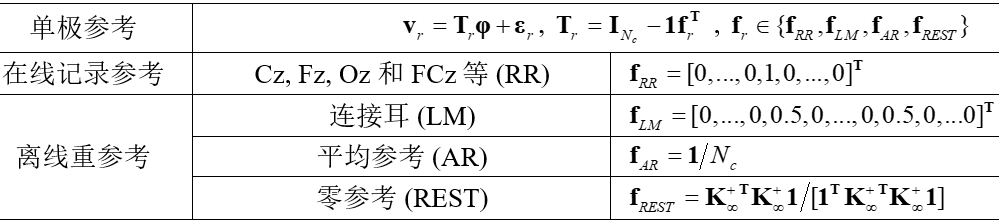
\includegraphics[width=\linewidth]{pic/ref3/table.png}
  \caption{单极参考家族。}
  \label{tab}
\end{table}

\section{REST作为单极参考的证明}\label{4:RESTasUR}
REST参考算子定义为
\begin{equation}\label{eq4.7}
\mathbf{T}_{REST}=\mathbf{K}_{\infty}\mathbf{K}_r^+\mathbf{T}_r
\end{equation}
这是脑电数据$\mathbf{v}_r$左乘$\mathbf{R}_r$\citing{hu_how_2018}。变换传递矩阵与\eqref{eq4.4}具有相同单极参考为
\begin{equation}\label{eq4.8}
\mathbf{K}_{r}=\mathbf{T}_r\mathbf{K}_{\infty}=\mathbf{K}_{\infty}+\mathbf{1}(\mathbf{-K}_{\infty}^T\mathbf{f}_r)^T
\end{equation}
因为分布神经源个数远大于电极数并考虑容积传导的异质性,$\mathbf{K}_{\infty}$所有行相互独立即行满秩,形成$\mathbf{K}_{\infty}\mathbf{K}_{\infty}^+=\mathbf{I}_{N_e}$以及$\rank(\mathbf{K}_r)=\rank(\mathbf{T}_r)$。 注意$\mathbf{T}_r$是满秩亏一\citing{hu_unified_2018}矩阵,因此$\rank(\mathbf{K}_r)=\rank(\mathbf{K}_{\infty})-1$正是论文\citing{baksalary_revisitation_2003}中理论1.1中的情形 ($\downarrow$)。通过论文\citing{baksalary_revisitation_2003}中的公式(1.3)定义$\mathbf{d}=-\mathbf{K}_{\infty}^+\mathbf{1}$得到
\begin{equation}\label{eq4.9}
\mathbf{K}_{r}^+\mathbf{K}_{r}=\mathbf{K}_{\infty}^+\mathbf{K}_{\infty}-\frac{\mathbf{dd}^T}{{\mathbf{d}^T\mathbf{d}}}=\mathbf{K}_{\infty}^+\mathbf{K}_{\infty}-\frac{\mathbf{K}_{\infty}^+\mathbf{11}^T\mathbf{K}_{\infty}^{+T}}{{\mathbf{1}^T\mathbf{K}_{\infty}^{+T}\mathbf{K}_{\infty}^+\mathbf{1}}}
\end{equation}
其推导可按照论文\citing{baksalary_revisitation_2003}中列表2.2中的情形($\downarrow$)得出。

\eqref{eq4.7}中的REST运算子右乘$\mathbf{K}_{\infty}\mathbf{K}_{\infty}^+=\mathbf{I}_{N_e}$,则REST变换算子成为
\begin{equation}\label{eq4.10}
\mathbf{T}_{REST}=\mathbf{K}_{\infty}\mathbf{K}_{r}^+\mathbf{K}_{r}\mathbf{K}_{\infty}^+=\mathbf{I}_{N_e}-\mathbf{1}\frac{\mathbf{1}^T\mathbf{K}_{\infty}^{+T}\mathbf{K}_{\infty}^+}{\mathbf{1}^T\mathbf{K}_{\infty}^{+T}\mathbf{K}_{\infty}^+\mathbf{1}}
\end{equation}
显然REST参考算子属于单极参考。写为形式$\mathbf{T}_{REST}=\mathbf{I}_{N_e}-\mathbf{1}\mathbf{f}_{REST}^T$,REST的线性变换权重
向量就为
\begin{equation}\label{eq4.11}
\mathbf{f}_{REST}={\mathbf{K}_\infty^+}^T\mathbf{K}_\infty^+\mathbf{1}/{[\mathbf{1}^T{\mathbf{K}_\infty^+}^T\mathbf{K}_\infty^+\mathbf{1}]}
\end{equation}

因此,REST运算子遵守\eqref{eq4.4}中单极参考家族的形式。 尽管参考标准化矩阵$\mathbf{R}_r$依赖数据中已应用的脑电参考,REST参考变换
算子$\mathbf{T}_{REST}$并不依赖脑电数据中特定的单极参考,注意$\mathbf{f}_r$在\eqref{eq4.11}中消失掉,所以无论\eqref{eq4.7}中使用哪个$\mathbf{T}_r$结果都一致。REST是单极参考的证明澄清了它本身与其它参考之间的关系。

\section{单极参考的属性}
分析单极参考家族发现一些重要属性,可以归纳为无记忆性,满秩减一和正交投影中心化。

\subsection{无记忆性}
假设$\mathbf{T}_{r1}=\mathbf{I}_{N_e}-\mathbf{1f}_{r1}^T$是最终想要应用的参考,$\mathbf{T}_{r2}$是此前已经应用在数据中的参考
,只要满足$\mathbf{f}_{r1}^T\mathbf{1}=1$就得到
\begin{equation}\label{eq4.12}
\mathbf{T}_{r1}=\mathbf{T}_{r1}\mathbf{T}_{r2}
\end{equation}
这里$\mathbf{T}_{r2}$可以是任意一种单极参考算子。

注意到$\mathbf{f}_r^T\mathbf{1}=1$对$\mathbf{f}_r\in{[\mathbf{f}_{RR},\mathbf{f}_{LM},\mathbf{f}_{AR},\mathbf{f}_{REST}]}$均成立。无记忆性对单极参考家族包括在线记录参考如Cz、Fz、Oz和FCz等及离线重参考如LM、AR和REST均成立。
\subsection{满秩减一性}
对于单极参考$\mathbf{T}_r$满足$\mathbf{f}_r\in{[\mathbf{f}_{RR},\mathbf{f}_{LM},\mathbf{f}_{AR},\mathbf{f}_{REST}]}$,都存
在
\begin{equation}\label{eq4.13}
\rank(\mathbf{T}_r)=N_e-1
\end{equation}
这意味着$\mathbf{T}_r$都是满秩减一。

\subsection{正交投影中心化属性} 
$\mathbf{T}_r^T$列空间上正交投影是中心化矩阵(等于平均参考)
\begin{equation}\label{eq4.14}
\mathbf{T}_r^+\mathbf{T}_r=\mathbf{T}_{AR}
\end{equation}
读者可以在论文\citing{hu_unified_2018}的附录中查看满秩减一和正交投影中心化的详细证明。

从\ref{4:RESTasUR}一节发现传递矩阵具有单位化属性$\mathbf{K}_{\infty}\mathbf{K}_{\infty}^+=\mathbf{I}_{N_e}$,满秩减一属性$\rank(\mathbf{K}_r)=\rank(\mathbf{K}_{\infty})-1$及正交投影中心化属性$\mathbf{K}_r^+\mathbf{K}_r=\mathbf{I}_{N_e}-\mathbf{K}_{\infty}^+\mathbf{11}^T\mathbf{K}_{\infty}^{+T}/{\mathbf{1}^T\mathbf{K}_{\infty}^{+^T}\mathbf{K}_{\infty}^+\mathbf{1}}$。如果传递矩阵$\mathbf{K}_{\infty}$是单位阵就很容易推出单极参考的满秩减一和正交投影中心化属性。然而实际中真实传递矩阵$\mathbf{K}_{\infty}$远非单位阵,传递矩阵的生物物理
学假设正是REST与其他单极参考存在区别的根本原因。

\section{AR和REST的最大似然估计}
寻找最优参考的实际目的是估计无穷远参考下的脑电电位而不是要真正找到无穷远处的参考信号。\eqref{eq4.3}中的单极参考模型可改写为块矩阵形式
\begin{equation}\label{eq4.15}
\begin{pmatrix}\mathbf{v}_{r-}\\v_r\end{pmatrix}=\begin{pmatrix}\mathbf{T}_{r-}\\\mathbf{t}_r^T\end{pmatrix}\mathbf{\phi}+\mathbf{\epsilon}_r
\end{equation}
这里$\mathbf{T}_{r-}\in\mathbb{R}^{(N_e-1)\times{N_e}}$是一个宽型矩阵,$\mathbf{t}_r\in\mathbb{R}^{N_e\times1}$,$\mathbf{v}_{r-}\in\mathbb{R}^{(N_e-1)\times1}$是向量,$v_r$是标量。

因为$\mathbf{T}_r$是满秩减一型,丢掉一行会得到行满秩矩阵。如果$\mathbf{T}_r$是记录参考,$\mathbf{t}_r$对应着物理参考电极。如果$\mathbf{T}_r$是左右连接乳突或者耳垂参考,$\mathbf{t}_r$对应着左右乳突或耳垂中的其中一个。

因此单极参考模型化为
\begin{equation}\label{eq4.16}
\mathbf{v}_{r-}=\mathbf{T}_{r-}\mathbf{\phi}+\mathbf{\epsilon}_{r-}
\end{equation}
这里$\mathbf{\epsilon}_{r-}$的协方差矩阵是$\Sigma_{\mathbf{\epsilon}_{r-}\mathbf{\epsilon}_{r-}}=\sigma^2\mathbf{T}_{r-}\mathbf{T}_{r-}^T$。

显然没有约束时,从$\mathbf{v}_{r-}\in\mathbb{R}^{(N_e-1)\times1}$估计$\mathbf{\phi}\in\mathbb{R}^{N_e\times1}$是欠定的问题。

平均参考(AR)的约束是
\begin{equation}\label{eq4.17}
\mathbf{1}^T\mathbf{\phi}=0
\end{equation}
其物理意义是分层球体且各向同性传导体表面的电位离散积分为零\citing{bertrand_theoretical_1985}。 对$\mathbf{\phi}$的估计是约束条件
下的线性回归问题。借助书籍\citing{magnus_matrix_2007}第303页中的定理6,对\eqref{eq4.16}的最优线性无偏估计量是
\begin{equation}\label{eq4.18}
\hat{\mathbf{\phi}}=(\mathbf{I}_{N_e-1}-\mathbf{P}^{-1}\mathbf{11}^T/{\mathbf{1}^T\mathbf{P}^{-1}\mathbf{1}})\mathbf{P}^{-1}\mathbf{T}_{r-}^T(\mathbf{T}_{r-}\mathbf{T}_{r-}^T)^{-1}\mathbf{v}_{r-}
\end{equation}
这里$\mathbf{P}={\mathbf{T}_{r-}^T(\mathbf{T}_{r-}\mathbf{T}_{r-}^T)^{-1}\mathbf{T}_{r-}}+\mathbf{11}^T$,因为$\mathbf{T}_{r-}^T(\mathbf{T}_{r-}\mathbf{T}_{r-}^T)^{-1}=\mathbf{T}_{r-}^+$以及$\mathbf{T}_{r-}^+\mathbf{T}_{r-}=\mathbf{T}_{AR}$。 $\mathbf{P}$就简化写作$\mathbf{P}=\mathbf{I}_{N_e-1}+\mathbf{11}^T/{[\mathbf{1}^T\mathbf{1}/(\mathbf{1}^T\mathbf{1}-1)]}$。

$\mathbf{P}$的矩阵广义逆可通过论文\citing{baksalary_revisitation_2003}中的公式(2.2)求解为
\begin{equation}\label{eq4.19}
\mathbf{P}^{-1}=\mathbf{I}-(\mathbf{1}^T\mathbf{1}-1)\mathbf{11}^T/{\mathbf{1}^T\mathbf{11}^T\mathbf{1}}
\end{equation}

将等式\eqref{eq4.19}代入等式\eqref{eq4.18}并简化得
\begin{equation}\label{eq4.20}
\hat{\mathbf{\phi}}=\mathbf{T}_{AR}\mathbf{T}_{r-}^+\mathbf{v}_{r-}=\mathbf{T}_{AR}\mathbf{T}_{r-}^+(\mathbf{T}_{r-}\mathbf{\phi}+\mathbf{\epsilon_{r-}})=\mathbf{T}_{AR}(\mathbf{\phi}+\mathbf{\epsilon})
\end{equation}
如果传感器电极噪声趋于零或被人为忽略,\eqref{eq4.20}就是传统的平均参考(AR)。 这说明通过约束所有电极电位和为零可推导出AR,如果该
约束正确且传感器电极噪声可忽略,无穷远参考下脑电电位的最优线性无偏估计量就是AR。

对于REST,将传递矩阵$\mathbf{K}_{\infty}$进行奇异值分解为$\mathbf{K}_{\infty}=\mathbf{USW}^T$,\eqref{eq4.16}表示为
\begin{equation}\label{eq4.21}
\mathbf{v}_{r-}=\mathbf{T}_{r-}\mathbf{USW}^T\mathbf{j}+\mathbf{\epsilon}_{r-}
\end{equation}
定义$\mathbf{L}=\mathbf{T}_{r-}\mathbf{US}$以及$\mathbf{\beta}=\mathbf{W}^T\mathbf{j}$,\eqref{eq4.21}化为
\begin{equation}\label{eq4.22}
\mathbf{v}_{r-}=\mathbf{L\beta}+\mathbf{T}_{r-}\mathbf{\epsilon}
\end{equation}

REST的约束是
\begin{equation}\label{eq4.23}
\min{\lVert{\beta}\rVert}_M^2
\end{equation}
这里$M$表示Mahalanobis距离。 这意味着REST不依赖特定溯源方法但依赖参数$\mathbf{\beta}=\mathbf{W}^T\mathbf{j}$。REST约束的是最小化正演模型(传递矩阵)和实际神经源活动信息组合起来的结构项。
因为$\mathbf{W}$是正交单位阵,当神经源活动$\mathbf{j}$具有独立同分布先验协方差时,$\mathbf{\beta}$的最小模等于$\mathbf{j}$的最小欧式模。

在等式\eqref{eq4.22}条件下求解约束\eqref{eq4.23}得到
\begin{equation}\label{eq4.24}
\hat{\mathbf{\beta}}=\Sigma_{\mathbf{\beta\beta}}\mathbf{L}^T(\mathbf{L}\Sigma_\mathbf{\beta\beta}\mathbf{L}^T+\mathbf{T}_{r-}\Sigma_{\mathbf{\epsilon\epsilon}}\mathbf{T}_{r-}^T)^{-1}\mathbf{v}_{r-}
\end{equation}

设等效源协方差为$\Sigma_\mathbf{jj}=\alpha^2\mathbf{I}_{N_s}$以及给定$\mathbf{K}_{r-}=\mathbf{T}_{r-}\mathbf{USW}^T$、$\mathbf{K}_{\infty}\mathbf{K}_{\infty}^T=\mathbf{US^2U}^T$,将\eqref{eq4.24}左乘$\mathbf{US}$得到
\begin{equation*}
\hat{\mathbf{\phi}}=\mathbf{K}_{\infty}\mathbf{K}_{r-}^T(\mathbf{K}_{r-}\mathbf{K}_{r-}^T+\frac{\sigma^2}{\alpha^2}\mathbf{T}_{r-}\mathbf{T}_{r-}^T)^{-1}\mathbf{v}_{r-}
\end{equation*}
当$\sigma$趋近零或传感器电极噪声被忽略,$\hat{\mathbf{\phi}}=\mathbf{K}_{\infty}\mathbf{K}_{r-}^+\mathbf{v}_{r-}$就是REST。
REST假设脑电电位由模拟容积传导效应的传递矩阵生成,可通过最小模约束对无穷远电位求解。

注意$\mathbf{K}_{\infty}$比$\mathbf{K}_{r-}$多一个通道表示REST的插值功能。 插值功能可在参考通道丢失恢复全通道记录或修复被丢弃坏道时使用。

\section{AR和REST的贝叶斯估计}
所有参考都是无穷远参考理想脑电电位的线性组合,通过传递矩阵转换为神经源活动的线性组合。因此$\hat{\mathbf{\phi}}$的估计转换为求解线性欠定逆问题,就有必要进行溯源研究。无穷远参考下脑电电位估计是
贝叶斯理论中的最大后验估计:
\begin{equation}\label{eq4.25}
P(\mathbf{\phi}\mid\mathbf{x},\mathbf{T}_o,\mathbf{\epsilon})\propto{P(\mathbf{x}\mid\mathbf{\phi},\mathbf{T}_o,\mathbf{\epsilon})P(\mathbf{\phi})P(\mathbf{\epsilon})}
\end{equation}
这里$P(\mathbf{\phi}\mid\mathbf{x},\mathbf{T}_o,\mathbf{\epsilon})$是给定似然$P(\mathbf{x}|\mathbf{\phi},\mathbf{T}_o,\mathbf{\epsilon})$和先验$P(\mathbf{\phi})$、$P(\mathbf{\epsilon})$的后验。使用调参$\lambda$,\eqref{eq4.25}按照书籍\citing{noauthor_mardia_nodate}可转换为
\begin{equation}\label{eq4.26}
\ell = \Vert\mathbf{x}-\mathbf{T}_o\mathbf{\phi}\rVert_M^2+\lambda\lVert\mathbf{\phi}\rVert_M^2
\end{equation}
解\eqref{eq4.26}得无穷远参考脑电电位的最大后验估计量
\begin{equation}\label{eq4.27}
\hat{\mathbf{\phi}}_o=\Sigma_\mathbf{\phi\phi}\mathbf{T}_o^T(\mathbf{T}_o\Sigma_\mathbf{\phi\phi}\mathbf{T}_o^T+\sigma^2\mathbf{T}_o\mathbf{T}_o^T)^+\mathbf{x}
\end{equation}
这是脑电参考问题的贝叶斯通解。指定脑电参考转换矩阵$\mathbf{T}_o$为$\mathbf{T}_r$,$\hat{\mathbf{\phi}}_o$估计量间的差异就
仅在于无穷远参考脑电电位的先验协方差$\Sigma_{\mathbf{\phi\phi}}$。

平均参考AR是等式\eqref{eq4.27}具有独立同分布先验协方差$\Sigma_{\mathbf{\phi\phi}}=\alpha^2\mathbf{I}_{N_e}$时的特例,可推出最
小模最小二乘解
\begin{equation}\label{eq4.28}
\hat{\mathbf{\phi}}_r=\alpha^2\mathbf{T}_r^T(\alpha^2\mathbf{T}_r\mathbf{T}_r^T+\sigma^2\mathbf{T}_r\mathbf{T}_r^T)^+\mathbf{v}_r
\end{equation}
当$\sigma^2$趋近于零,代\eqref{eq4.3}入\eqref{eq4.28}并简化为
\begin{equation}\label{eq4.29}
\hat{\mathbf{\phi}}_r=\mathbf{T}_r^+\mathbf{T}_r\mathbf{\phi}+\mathbf{T}_r^+\mathbf{\epsilon}_r
\end{equation}

正交投影中心化属性对单极参考家族都成立,因此
\begin{equation}\label{eq4.30}
\hat{\mathbf{\phi}}_{AR}=\hat{\mathbf{\phi}}_r=\mathbf{T}_{AR}\mathbf{\phi}+\mathbf{\epsilon}_{AR}
\end{equation}
当$\mathbf{\phi}$是独立同分布,任何单极参考下\eqref{eq4.3}的最小模解都是平均参考(AR),验证了AR只能用于之前被参考于其它单极参考的脑电数据这一推断\citing{hu_restate_2018}。

如果无穷远参考脑电电位$\mathbf{\phi}$由独立同分布先验协方差的神经源活动生成,就能推出REST。对于任何参考下的脑电数据,\eqref{eq4.2}的变形都成立:
\begin{equation}\label{eq4.31}
\mathbf{x}=\mathbf{T}_o\mathbf{\phi}+\mathbf{\epsilon}_o=\mathbf{K}_o\mathbf{j}+\mathbf{\epsilon}_o
\end{equation}

这里$\mathbf{K}_o=\mathbf{T}_o\mathbf{K}_{\infty}$是线性变换后的正演模型。设等效源协方差为$\Sigma_{\mathbf{jj}}$,则等式\eqref{eq4.31}的解表示为
\begin{equation}\label{eq4.32}
\hat{\mathbf{\phi}}_{rREST}=\mathbf{K}_{\infty}\Sigma_{\mathbf{jj}}\mathbf{K}_o^T(\mathbf{K}_o\Sigma_{\mathbf{jj}}\mathbf{K}_o^T+\sigma^2\mathbf{T}_r\mathbf{T}_r^T)^+\mathbf{x}
\end{equation}
这是REST的正则化版本rREST\citing{hu_unified_2018}。 假设等效源具有独立同分布协方差先验$\Sigma_\mathbf{jj}=\alpha^2\mathbf{I}_{N_s}$,rREST参考算子简化为
\begin{equation}\label{eq4.33}
\mathbf{T}_{rREST}=\alpha^2\mathbf{K}_{\infty}\mathbf{K}_o^T(\alpha^2\mathbf{K}_o\mathbf{K}_o^T+\sigma^2\mathbf{T}_o\mathbf{T}_o^T)^+
\end{equation}

当通过单极参考$r$变换得到$\mathbf{x}$,$\sigma$趋近于零(无噪声数据),\eqref{eq4.33}就简化为传统REST\citing{yao_method_2001}。

通过贝叶斯理论,REST假设脑电电位由独立神经源生成\citing{hu_unified_2018}。神经源其它类型协方差先验对REST型估计量的影响还在研究中。 
\section{讨论}
本章脑电参考问题的广义形式被理解为无穷远参考脑电电位$\mathbf{\phi}$的线性转换,可能是单极参考或者非单极参考如双极记录或头表拉普拉斯变换;统一数学表达式给出单极参考的共同结构;首次发现解决参考问题的插值功能并证明REST是一种单极参考。这允许研究单极参考家族及其规律。还归纳出单极参考家族的一些属性以建立它们的内在联系。

出乎意料的属性是无记忆性,表明单极参考独立起作用不受已应用单极参考的影响,意味着总可以安全地用不同参考技术重新参考脑电或者诱发电位记录但无需担心多次重参考会累积误差,任何两个单极参考可以相互转换,所有的单极参考相互独立起作用。 转换为另一个单极参考前需要确认目前数据是基于单极参考,从非单极参考到单极参考的转换会破坏数据集。该属性表明单极参考可消除其他单极参考的影响,多次应用单极参考是安全的。实际脑电数据预处理中,无记忆性值得被脑电研究工作者注意到。

秩亏一这一具有显著意义的属性意味着单极参考总将无穷远参考下的理想脑电电位的满秩减一。丢失掉的秩是因为从所有电极上减去的参考信号是所有电极在无穷远参考下活动的线性组合。该属性说明不引入额外先验信息就不可能获得对理想脑电电位$\mathbf{\phi}$的无偏估计。不同单极参考的确具有不同偏差,依赖于估计无穷远理想电位$\mathbf{\phi}$时用到多少先验信息。

正交投影中心化这一重要属性从满秩减一型矩阵的Moore–Penrose伪逆理论证明得到。该属性在最大似然估计和贝叶斯理论推导AR过程中得到充分使用。REST用的传递矩阵具有正交投影加权中心化属性。和单位化属性及秩减一属性一起,REST被证明为一种单极参考。正是借助这种正交投影(加权)中心化属性才证明AR和REST不依赖以前应用于脑电数据上的任何具体单极参考,最终都可推出AR和REST。

单极参考家族中AR和REST是两个主要竞争对手。本章发现最大似然估计和贝叶斯理论方法都可推出AR和REST。一种方法是利用广义线性回归模型\citing{magnus_matrix_2007}使用最大似然估计,分别用线性和二次约束项推导出AR和REST。给定所有电极上脑电电位和为零的线性约束可证明AR是最优线性无偏估计量。相比,REST是最小化等效源线性结合的二次约束。更灵活的推导是利用贝叶斯理论,通过假设多通道脑电记录具有先验的独立同分布协方差可推出AR;通过容积传导模型和神经源活动的先验独立同分布协方差可推出REST。从最大似然估计的角度,如果头皮脑电电位的离散积分为零的约束正确,AR就是理论正确解。无论从哪个单极参考开始,最佳无偏线性估计量都是AR。电位积分部分程度上依赖电极分布和密度\citing{bertrand_theoretical_1985,nunez_rest_2010}。但第二章研究表明AR与电极密度并无紧密联系,和基于零积分假设的常规理解
不同,覆盖范围是比电极密度更重要的因素\citing{hu_how_2018}。 从贝叶斯角度发现AR实质上是在解广义线性逆问题来估计无穷远参考下的电位。无论脑电数据基于哪种单极参考用多通道脑电电位独立同分布的先验假设,最小模估计量的结果都是AR。因为容积传导效应,无穷远参考下多通道脑电电位独立同分布协方差先验的假设确定是错的。转换为AR前还要确认手头的脑电数据基于一种单极参考,限制了AR的使用范围\citing{hu_restate_2018}。

从最大似然估计的角度看,二次约束表明REST不完全依赖源空间的配置但依赖通过代表无限多源配置的等效源投影到头表活动的效果。假设脑电数据由大脑神经源生成时,理论上rREST是无穷远参考脑电电位的最优估计。REST允许正演计算中的电极数比估计等效源时用到的电极数多。正演模型中更多的电极数表明那些丢失或被拒绝的坏道可通过REST的插值功能恢复。

REST中神经源的统计学分布仅是无穷远电位估计中的一种特殊先验,REST是一种最大后验估计量,其等效源方法可防止对源的错误估计。REST的目标不是找到实际神经源也不必需。作为REST的扩展,rREST具有更加广泛应用的能力。公式\eqref{eq4.31}-\eqref{eq4.33}是广义的,不管哪种$\mathbf{T}_o$应用到$\mathbf{x}$,rREST都能适应非单极参考的记录如双极记录和头拉普拉斯。REST可能的两个限制是无噪声脑电数据的
假设和球面头模型的使用。仿真研究和大量真实脑电数据表明除非脑电数据具有极高的SNR,使用球面传递矩阵的REST就可以,无需构造真实头模型。被试群体平均的传递矩阵和基于广义交叉验证的去噪应在rREST实际中应用\citing{hu_unified_2018}。读者可以访问https://github.com/ShiangHu/LeadField-Pipeline获得易于计算实际头模型的流程代码和https://github.com/ShiangHu/Unified-EEG-reference-rREST了解如何使用rREST。
\section{本章小结}
本章发现包括REST在内所有常见脑电参考都可用统一数学符号表示为单极参考家族。单极参考的一些属性如无记忆性、满秩亏一、正交投影中心化可能在帮助实际运用参考中具有重要价值。最大似然估计和贝叶斯理论
都推导出AR和REST。这些结果加上REST的插值功能,为将来定量脑电分析中参考的使用提供了崭新理解。